%-------------------------------------------------------------------------------
%	CAPITOLO 20
%-------------------------------------------------------------------------------

\chapter{Gli artigiani}

A dire il vero in Alfonsine non furono molti, si ricorda una epigrafe\footnote{Testo esposto pubblicamente su un supporto di materiale non deperibile} che andò per varie generazioni e cioè:
\\\\
\textcal \Huge
	\centerline{Gramantieri Tomaso}
	\centerline{e car fasè}
	\centerline{Santoni Proculo}
	\centerline{ul piturè}\normalfont \normalsize \footnote{\textbf{Tomaso Gramantieri} fece il carro, \textbf{Proculo Santoni} lo pitturò - Mi è stato detto da \index[Personaggi]{Pasi Adis}Adis Pasi che in una casa dietro alla \index[Luoghi]{Villa Marini}Villa Marini, vi era questa epigrafe che però riportava una frase leggermente diversa: "Checco Gramantieri e car fasè, Brocul e Santoni il piturè"}

\index[Personaggi]{Gramantieri Tomaso}\index[Personaggi]{Santoni Proculo}

 \begin{figure}[htb]
    \centering
    \vspace{-0.3cm}
    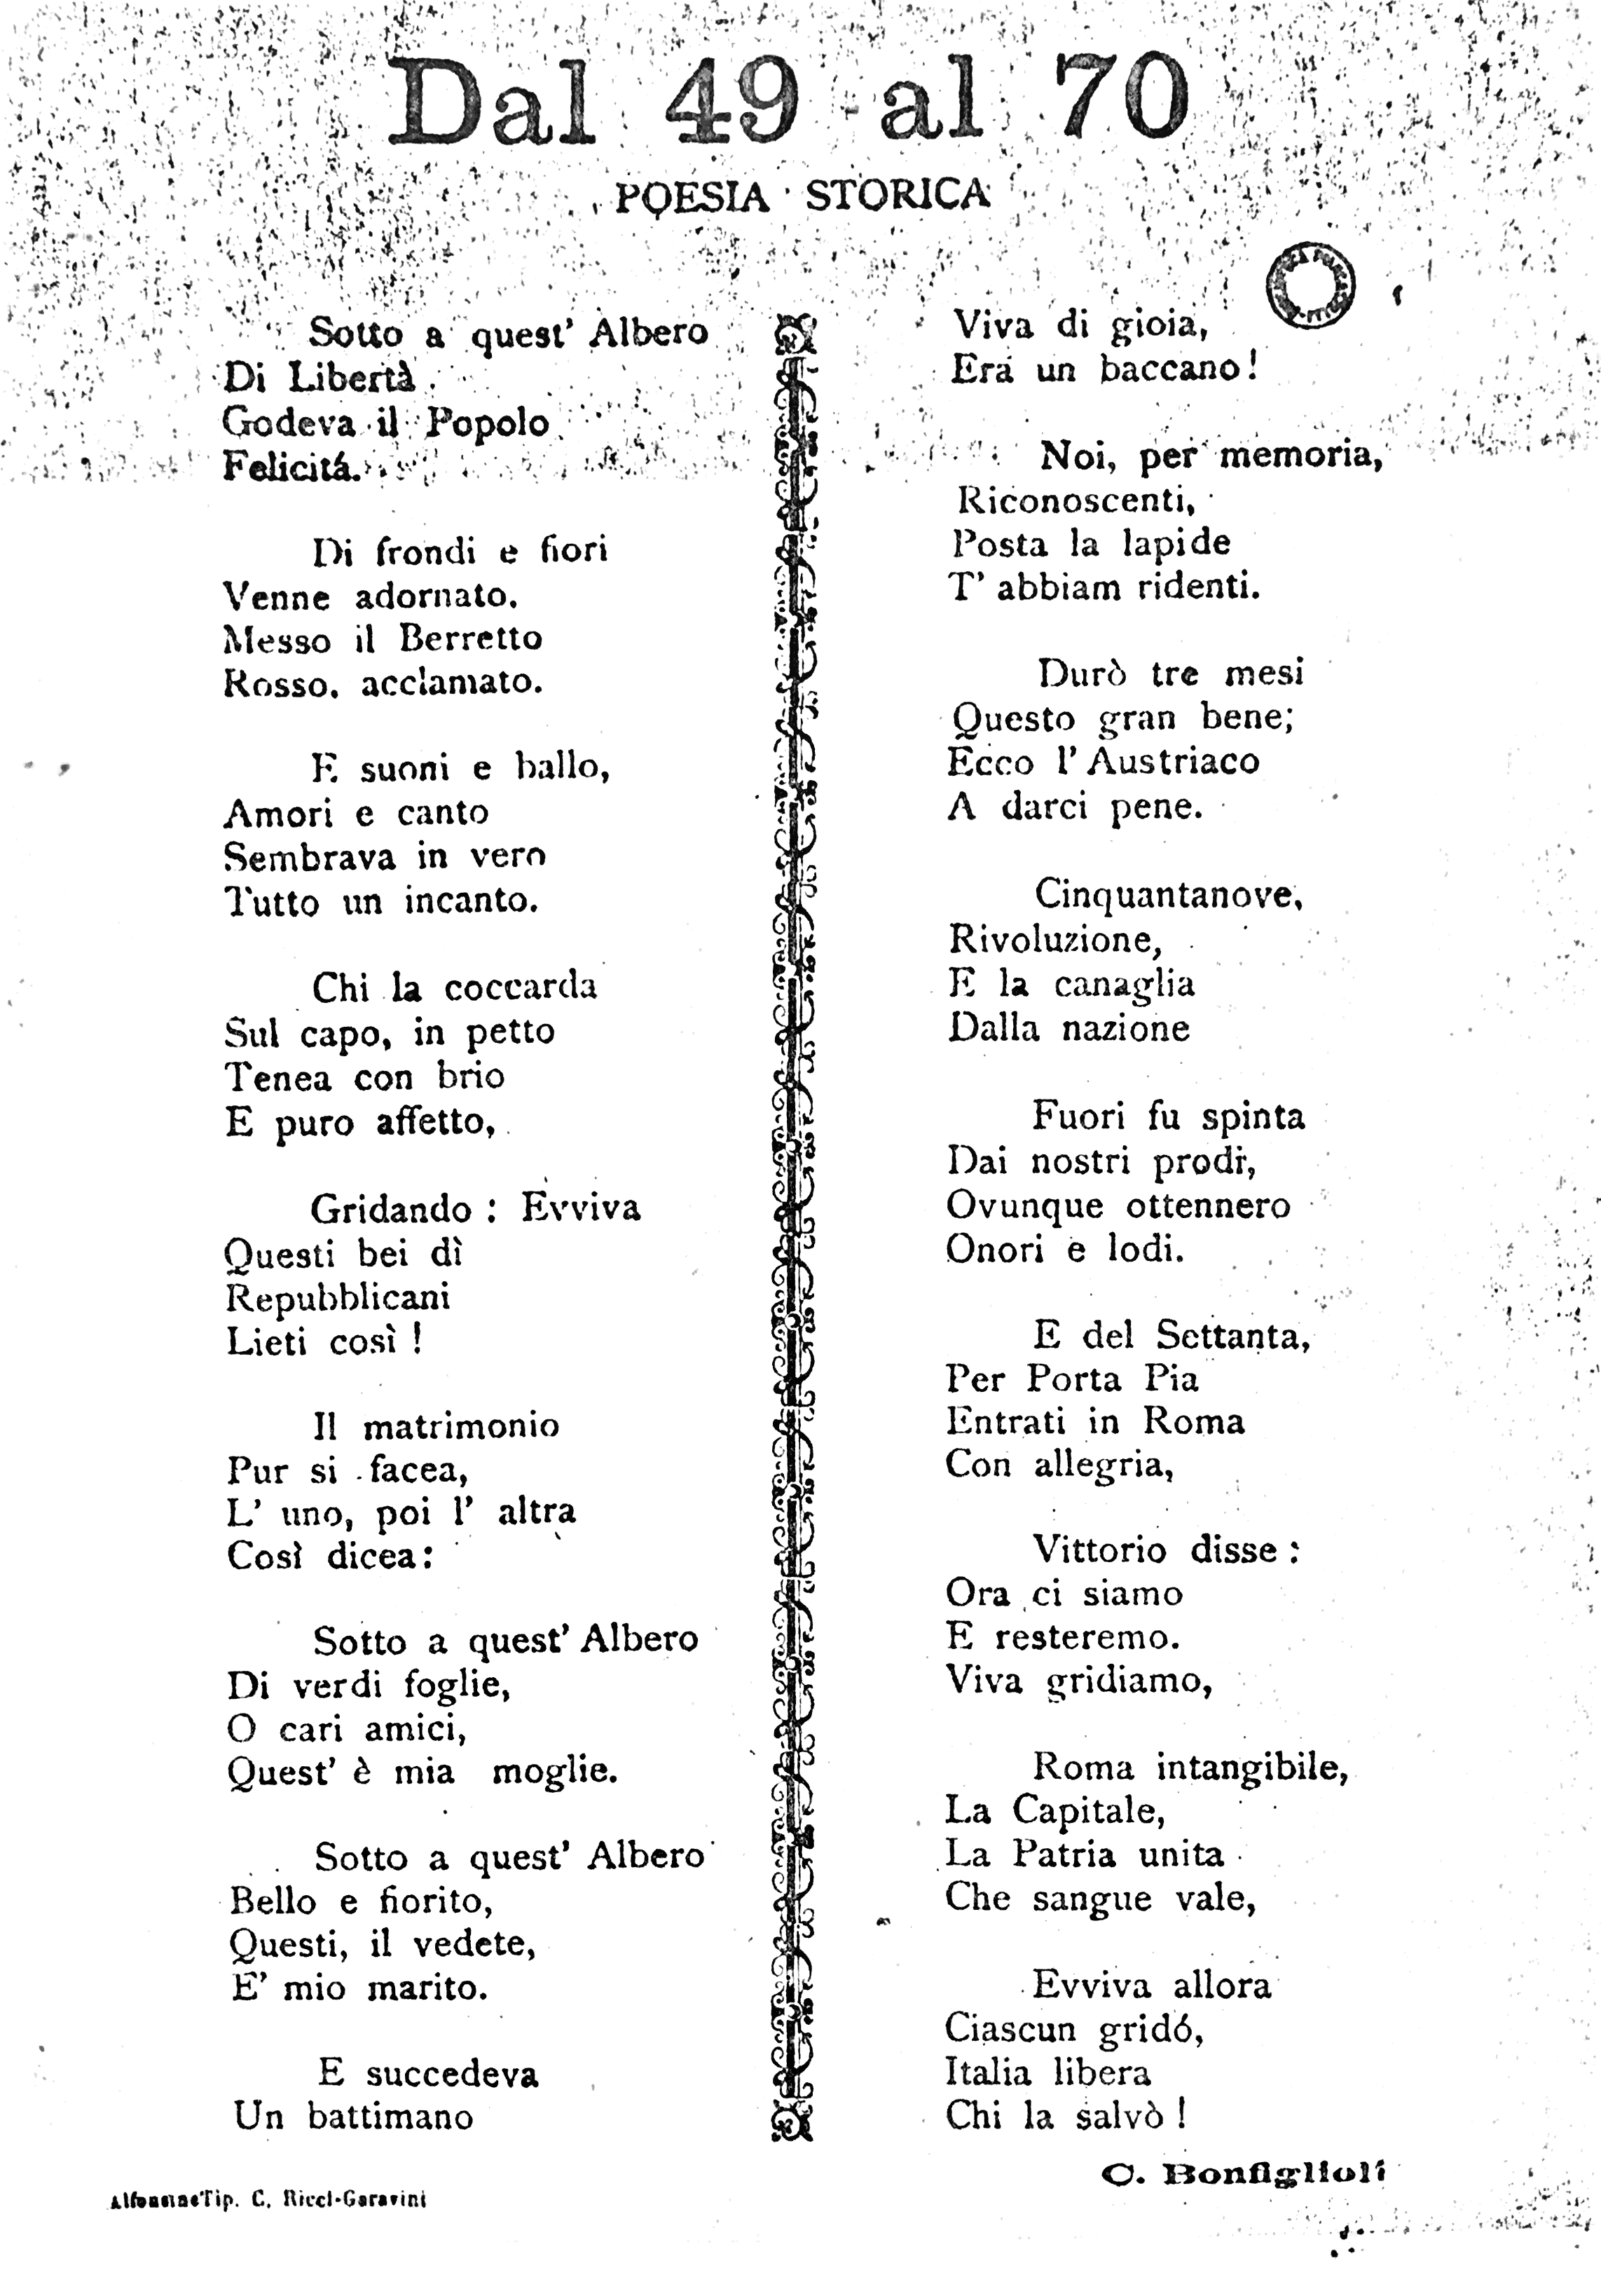
\includegraphics[width=\textwidth]{ciro}
    \caption[Poesia Ciro Bonfiglioli]{Una poesia di \textbf{Ciro Bonfiglioli}\index[Personaggi]{Bonfiglioli Ciro} che ho trovato nell'archivio storico di Alfonsine, nella biblioteca P. Orioli.\label{fig:ciro}}
    \vspace{-0.7cm}
\end{figure}


